\documentclass[a4paper,10pt,fleqn,twocolumn]{IEEEtran}

\usepackage{amsfonts}
%\usepackage{amsthm}
\usepackage{graphicx}


%\newtheorem{Prop}{Proposition}
%\newtheorem{lemma}{Lemma}
%\newtheorem{Proof}{proof}

\newcommand{\br}{{\mathbf r}}
\newcommand{\bA}{{\mathbf A}}
\newcommand{\ba}{{\bf a}}
\newcommand{\bb}{{\bf b}}
\newcommand{\bs}{{\bf s}}
\newcommand{\bn}{{\bf n}}
\newcommand{\bv}{{\bf v}}
\newcommand{\bu}{{\bf u}}
\newcommand{\bw}{{\bf w}}
\newcommand{\bx}{{\bf x}}
\newcommand{\by}{{\bf y}}
\newcommand{\bbf}{{\bf f}}
\newcommand{\bS}{{\bf S}}
\newcommand{\bN}{{\bf N}}
\newcommand{\bD}{{\bf D}}
\newcommand{\bX}{{\bf X}}
\newcommand{\bY}{{\bf Y}}
\newcommand{\bZ}{{\bf Z}}
\newcommand{\bP}{{\bf P}}
\newcommand{\bI}{{\bf I}}
\newcommand{\bR}{{\bf R}}
\newcommand{\bU}{{\bf U}}
\newcommand{\bV}{{\bf V}}
\newcommand{\bW}{{\bf W}}
\newcommand{\bJ}{{\bf J}}
\newcommand{\bB}{{\bf B}}
\newcommand{\bcS}{{\bf {\cal S}}}
\newcommand{\bcH}{{\bf {\cal H}}}
\newcommand{\bzero}{{\bf 0}}
\newcommand{\bgamma}{{\mbox {\boldmath $r$}}}
\newcommand{\btheta}{{\mbox {\boldmath $\theta$}}}
\newcommand{\bLambda}{{\mbox {\boldmath $\Lambda$}}}
\newcommand{\bPsi}{{\mbox {\boldmath $\Psi$}}}
\newcommand{\bPhi}{{\mbox {\boldmath $\Phi$}}}
\newcommand{\bcI}{{\mbox {\boldmath ${\cal I}$}}}
\newcommand{\bcR}{{\mbox {\boldmath ${\cal R}$}}}
\newcommand{\bcB}{{\mbox {\boldmath ${\cal B}$}}}


\title{Joint Direction and Frequency Estimation With Small-Array Receiver}
\author{{Shu Wang, James Caffery, Jr. and Hanhong Shen} \\ Department of ECECS \\ University of Cincinnati \\Cincinnati, OH 45221-0030}
%\date{}
%\pagestyle{plain}
\begin{document}
\maketitle
\begin{abstract}
Several high-resolution subspace schemes for jointly estimating
the direction and frequency of each arriving signal with a small
ESPRIT array receiver are presented, in which the physical size of
array is smaller than the number of signals. Following the concept
of the conventional ESPRIT algorithm, a special signal parameter
matrix is constructed so that the direction and frequency of each
signal are estimated directly from its eigenvalue and eigenvector
pair. No searching or pairing procedure is necessary. With further
analysis of the correlation matrix properties, some enhancements
with space-time preprocessing and total least squared estimation
are given. Besides that the Cram\'er-Rao lower bound is given for
performance discussion , the first-order approximation of the
asymptotic mean squared estimation errors is also derived and
discussed. Computer simulations are presented to demonstrate the
performance of the proposed schemes.
\end{abstract}
\section{Introduction}
The application of antenna array is expected to help reduce
co-channel interference, extend coverage, increase spectral
efficiency and therefore fulfill increasing demands for higher
capacity and more services from the existing or next-generation
wireless communication systems~\cite{Ghav05,Dohl07}. With array
signal processing, both transmitter and receiver can benefit from
better channel estimation, more accurate signal steering and less
interference~\cite{Ghav05}. With multiple-antenna transmission,
higher spectrum efficiency is achievable without increasing
transmit power~\cite{Dohl07}. In these applications,
high-resolution signal parameter estimation, e.g., direction or
frequency-of-arrival (DOA/FOA) estimation, within the output data
of an array of antennas at different locations in space and/or
time domain of a wave-field is frequently studied~\cite{Ghav05}.
Roy et al. proposed a patented subspace rotation approach, ESPRIT,
for signal parameter estimation, which can be used for finding the
direction or frequency in a computationally efficient
manner~\cite{Roy89}. It is search-free and fairly robust with no
array calibration information and its performance is close to the
calibrated Cram\'er-Rao lower bound (CRLB) for many cases of
practical interest~\cite{Roy89}. All these make it very
competitive with many other algorithms~\cite{Ghav05}.

Though the generalization of so-called high-resolution one
dimensional (1D) algorithms to two-dimensional (2D) cases is
relatively straightforward, the main difficulty associated with
these methods is that both computation and storage costs tend to
increase rapidly with the number of dimensions of the parameter
vector due to searching~\cite{Zolt96,Wong97,Bro98} and possible
non-trivial pairing procedures~\cite{Chen92,Veen92,Kedi96}. Since
those high-resolution 2D methods have a considerably higher
computational cost, many implementations employ non-parametric
techniques in practice, e.g., Butler beam scanning. These
non-parameteric techniques are less complicated but their
performance is known to be poor~\cite{Goda97}. Additionally, most
modern high-resolution techniques require that the antenna array
size must be greater than the number of signal sources to avoid
ambiguity problem. This, in turn, may further render the
applicability of these techniques unattractive~\cite{Wang98}. And
this also make it a very important topic to design the receivers
tracking many more signal sources than the employed array size and
also understand the tradeoffs between array size and estimation
accuracy.

In this paper, several joint direction and frequency estimation
algorithms using small ESPRIT array are presented and discussed,
where the antenna array consists of several doublets the number of
which is less than the number of tracked signals. Different to
conventional ESPRIT and other 2D high-resolution estimation
approaches, a special signal parameter matrix is constructed with
each eigenvalue/eigenvector pair associated the
direction/frequency of a tracked signal. This makes the proposed
algorithms computation efficient with no search or pairing
procedure necessary and attractive for practical implementation.
Besides this, with additional analysis of the estimation of
involved correlation matrices, two enhancements are outlined too.
One enhancement is to perform a space-time preprocessing on
correlation matrix and the other one is to improve the signal
parameter estimation accuracy with total least squared (TLS)
estimation instead of the regular least squared (LS) estimation.
In addition to the formulation of the 2D CRLB on our approaches,
an asymptotic analysis of the estimation performance with
first-order approximation is given. Compared with the 2D CRLB,
this asymptotic analysis is more algorithm-specific and accurate.
It also gives more insights of the proposed algorithms. Computer
simulations are also presented to support our conclusions.
\section{System Model And Problem Description}
Let's assume there are $K$ uncorrelated narrow-band radiating
sources which emit plane wave signals, $s_{k}(t)$, with different
center frequencies, $f_{k}$, from distinct directions,
$\theta_{k}$, $k=1$, $2$, $\ldots$, $K$, corrupted by a additive
Gaussian white noise (AWGN) with variance, $\sigma^2$, at the
array receiver. This is a typical scenario happened in most
wireless communication, especially in the reverselink. We assume
that the plane waves and additive noise are stationary zero-mean
processes and uncorrelated from sensor to sensor. The complex form
of the observed signal $r_{m}\left(t\right)$ at the $m$th antenna
element of the array can be expressed as
\begin{equation}
\begin{array}{rcl}
r_{m}\left(t\right)&=&\sum\limits_{k=1}^Ka_{m}\left(f_{k},\
\theta_{k}\right)s_{k}\left(t\right)e^{-j2\pi
f_{k}t}+n_{m}\left(t\right)
\end{array}\label{ScaleModel}
\end{equation}
\noindent where $a_{m}\left(f_{k},\ \theta_{k}\right)$ denotes the
complex response, including both the gain
$g_{m,k}=\left|a_{m}\left(f_{k},\ \theta_{k}\right)\right|$ and
the phase $\phi_{m,k}={\rm arg}\left\{a_{m}\left(f_{k},\
\theta_{k}\right)\right\}$, of antenna $m$ at frequency $f_{k}$
and direction $\theta_{k}$, $s_{k}\left(t\right)$ is the
narrow-band signal and the size of array receiver is $M$. The
observed array signal samples can also be expressed in time-domain
vector and matrix form as
\begin{equation}%\hspace{-0.19in}
\begin{array}{rcl}
\br_{\rm T}^{(m)}\left(t\right)&=&\left[r_{m}\left(t\right)\ \cdots\ r_{m}\left(t+\left(L-1\right)T_{s}\right)\right]^{\rm T}\\
&=&\bA_{\rm T}^{\ast}\bs\left(t\right)+\bn_{\rm
T}^{(m)}\left(t\right)
\end{array} \label{VectorModelT}
\end{equation}
\noindent and
\begin{equation}
\begin{array}{rcl}
\bcR\left(t\right)&=&\left[\br_{\rm T}^{(1)}\left(t\right)\
\br_{\rm T}^{(2)}\left(t\right)\ \cdots\
\br_{\rm T}^{(M)}\left(t\right)\right]^{\rm T}\\
&=&\bA_{\rm S}\bS\left(t\right)\bA_{\rm T}^{\rm
H}+\bN\left(t\right)
\end{array} \label{MatrixModel}
\end{equation}
\noindent where $\br_{\rm T}^{(m)}\left(t\right)$ is a $L\times 1$
vector of $L$ consecutive samples at the $m$th antenna.
$\bcR\left(t\right)$ is the $M\times L$ signal matrix constructed
with the temporal signal vectors $\{\br_{\rm
T}^{(m)}\left(t\right):\ t=0,\ 1,\ \ldots,\ L-1\}$. The parameter
$T_{s}=\frac{1}{f_{s}}$ denotes the sample period which is the
inverse of the sampling frequency, $f_s$,
$\left[\cdot\right]^{\ast}$ denotes the complex conjugate
operator, $\left[\cdot\right]^{\rm T}$ denotes the transpose
operator and $\left[\cdot\right]^{\rm H}$ denotes the complex
conjugate transpose operator. In (\ref{MatrixModel}),
$\mathbf{A}_{\rm S}$ is labelled as $M\times K$ {\em spatial
steering matrix} written by
\begin{equation}
\begin{array}{rcl}
\bA_{\rm S}&=&\left[\ba_{\rm S}\left(f_{1},\theta_{1}\right)\
\ba_{\rm S}\left(f_{2},\theta_{2}\right)\ \cdots\ \ba_{\rm
S}\left(f_{K},\theta_{K}\right)\right]
\end{array},
\end{equation}
\noindent of which the $k$th column $\ba_{\rm S}\left(f_{k},\
\theta_{k}\right)$ denotes the $M\times 1$ {\em spatial steering
vector}, defined by
\begin{equation}
\begin{array}{rcl}
\ba_{\rm S}\left(f_{k},\
\theta_{k}\right)&=&\left[a_{1}\left(f_{k},\ \theta_{k}\right)\ \
\cdots\ \ a_{M}\left(f_{k},\ \theta_{k}\right)\right]^{\rm T}
\end{array}\label{a_S}
\end{equation}
\noindent for the $k$th arriving wave-front $s_{k}\left(t\right)$.
Likewise, $\bA_{\rm T}$ is labelled as $L\times K$ {\em temporal
steering matrix} expressed by
\begin{equation}
\begin{array}{rcl}
\bA_{\rm T}&=&\left[\ba_{\rm T}\left(f_{1}\right)\ \ba_{\rm
T}\left(f_{2}\right)\ \cdots\ \ba_{\rm T}\left(f_{K}\right)\right]
\end{array},
\end{equation}
\noindent of which the $k$th column
\begin{equation}
\begin{array}{rcl}
\ba_{\rm T}\left(f_{k}\right)&=&\left[1\ \
e^{j2\pi\frac{f_{k}}{f_{s}}}\ \ e^{j4\pi\frac{f_{k}}{f_{s}}}\
\cdots\ \ e^{j2\pi (L-1)\frac{f_{k}}{f_{s}}}\right]^{\rm T}
\end{array}\label{a_T}
\end{equation}
\noindent is a $L\times 1$ {\em temporal steering vector}. In
(\ref{VectorModelT}) and (\ref{MatrixModel}), $\bs\left(t\right)$
and $\bS\left(t\right)$ are the $K\times 1$ signal vector and
$K\times K$ signal diagonal matrix, respectively defined by
\begin{equation}
\begin{array}{rcl}
\bs\left(t\right)&=&\left[s_{1}\left(t\right)\
s_{2}\left(t\right)\ \ldots\ s_{K}\left(t\right)\right]^{\rm T}
\end{array}
\end{equation}
\noindent and
\begin{equation}
\begin{array}{rcl}
\bS\left(t\right)&=&\mbox{diag}\left\{\left[s_{1}\left(t\right)\
s_{2}\left(t\right)\ \ldots\ s_{K}\left(t\right)\right]\right\}
\end{array},
\end{equation}
\noindent for the $K$ carrier signals. $\bn_{\rm
T}^{(m)}\left(t\right)$ and $\bN\left(t\right)$ are the
corresponding $L\times 1$ noise vector and $M\times L$ noise
matrix, respectively.

The DOA/FOA estimation problem is to estimate the
direction-frequency pairs $\{\left(f_{k},\ \theta_{k}\right):\
k=1,\ 2,\ \ldots,\ K\}$, providing (\ref{VectorModelT}) and
(\ref{MatrixModel}) are available. This can be done with some
linear signal processing approaches, such as Butler beam scanning
or 2D Fourier spectrum analysis on received signals
$\{r_{m}\left(t\right):\ 1\leq m\leq M \}$. However, the
resolution of these linear approaches typically may not be good
high enough for many applications. Here we propose several
high-resolution signal parameter estimation approaches with signal
spectrum analysis and a small ESPRIT array. Compared with other
popular array structures like uniform linear array (ULA) and
uniform circular array (UCA), ESPRIT array consisting of multiple
doublets has flexible structure and does't require calibration
between doublets. This makes it very attractive for practical
deployment. Besides this, most wireless system is required to
serve more users with a small-size array in reality. This becomes
more critical when the system operates in a large number of
frequency bands. This is because of not only the large number of
users being simultaneously served but also the size limitation of
most receivers. Therefore, it is very important to estimate signal
parameters using small array and understand the tradeoff between
array size and estimation accuracy.
\section{Joint DOA/FOA Estimation with ESPRIT Array}
We assume a simple uncalibrated ESPRIT array consisting of two
subsarrys $\cal X$ and $\cal Y$ of the same size $M$. They are
identical and separated by a fixed distance $d$. Each pair of
identical elements of these two subarrays may be called {\em
doublet}. The directional gain and phase response of these
doublets may be completely different. This requirement makes the
necessary array calibrate much easier in reality. The relationship
between the carrier signals received by subarray $\cal X$ and
$\cal Y$ is
\begin{equation}
\begin{array}{rcl}
\bS^{x}\left(t\right)&=&\bS^{y}\left(t\right)\bD_{\rm S}
\end{array}
\end{equation}
\noindent where $\bS^{x}\left(t\right)$ and
$\bS^{y}\left(t\right)$ denote the signal matrix
$\bS\left(t\right)$ received by subarray $\cal X$ and $\cal Y$ at
time $t$, respectively, and
\begin{equation}
\begin{array}{rcl}
\bD_{\rm S}&=&\mbox{diag}\left\{\left[e^{j2\pi
f_{1}\frac{d\sin\theta_{1}}{c}}\ \cdots\ e^{j2\pi
f_{K}\frac{d\sin\theta_{K}}{c}}\right]\right\}
\end{array} \label{D_S}
\end{equation}
\noindent denotes the spatial rotation diagonal matrix, which
includes the information of the direction-frequency pairs
$\{\left(f_{k},\ \theta_{k}\right):\ k=1,\ 2,\ \ldots,\ K\}$. In
order to obtain the high-resolution estimation of the
direction-frequency pairs, it is necessary to analysis the signal
spectral structure of (\ref{MatrixModel}). For this, the
time-domain correlation matrices of the outputs of subarray $\cal
X$ and $\cal Y$ can be expressed by
\begin{equation}\hspace{-0.14in}
\begin{array}{rcccl}
\bR_{\rm T}^{xx}&=&\frac{1}{M}\mbox{E}\left\{\bX^{\rm
H}\left(t\right)\bX\left(t\right)\right\}&=&\bA_{\rm
T}\bP_{s}\bA_{\rm T}^{\rm H}+\sigma^2\bI
\end{array} \label{CorrelationXX}
\end{equation}
\noindent and
\begin{equation}
\begin{array}{rcccl}
\bR_{\rm T}^{yx}&=&\frac{1}{M}\mbox{E}\left\{\bY^{\rm
H}\left(t\right)\bX\left(t\right)\right\} &=&\bA_{\rm
T}\bP_{s}\bD_{\rm S}\bA_{\rm T}^{\rm H}
\end{array} \label{CorrelationXY}
\end{equation}
\noindent where $\bX$ and $\bY$ denote the signal matrix $\bcR$
received by subarray $\cal X$ and $\cal Y$, respectively.

With (\ref{CorrelationXX}) and (\ref{CorrelationXY}), a special
signal parameter matrix $\bR$ is defined by
\begin{equation}
\begin{array}{rcccl}
\bR&=&\mathbf{\bar{R}}_{\rm T}^{xx+}\bR_{\rm
T}^{yx}&=&\left(\bR_{\rm T}^{xx}-\sigma^2\bI\right)^{+}\bR_{\rm
T}^{yx}
\end{array}\label{RLS}
\end{equation}
\noindent with $\mathbf{\bar{R}}_{\rm T}^{xx}=\bR_{\rm
T}^{xx}-\sigma^2\bI$ denoting the correlation matrix of subarray
$\cal X$ or $\cal Y$ with no noise. Furthermore, when the ranks of
$\bA_{\rm T}$ and $\bP_{s}$ are $K$, the $k$th column of the
temporal steering matrix $\bA_{\rm T}$ is the eigenvector of the
signal parameter matrix $\bR$, which in turn corresponds to the
$k$th diagonal element of the diagonal matrix $\bD_{\rm S}$. This
can be expressed by
\begin{equation}
\begin{array}{rcl}
\bR\bA_{\rm T}&=&\bA_{\rm T}\bD_{\rm S}
\end{array}.\label{LS}
\end{equation}

With (\ref{LS}), the frequency and direction of each signal source
can be estimated from one pair of an eigenvector and a nonzero
eigenvalue. As a result, they are automatically coupled. No
additional search or pairing procedure is necessary. No knowledge
of the subarray responses is required, either. Furthermore, we can
see that, in (\ref{RLS}), the size of the square matrix $\bR$ is
$M$, which can be set to an arbitrary number regardless of the
physical array size. This means that even with a single doublet,
it is still possible to estimate as many incoming signals as
desired, provided that there are enough array measurements
available. Finally, the question left is how to estimate the
signal parameter matrix $\bR$ with the estimates $\tilde{\bR}_{\rm
T}^{xx}$ and $\hat{\bR}_{\rm T}^{yx}$ of the correlation matrices
defined in (\ref{CorrelationXX}) and (\ref{CorrelationXY})
available. Here two estimation schemes, LS estimation and TLS
estimation, and one pre-processing enhancement are presented.
\subsection{Least Squares Estimation}
The least square estimation of $\bR$ is the solution to the
following optimization problem and can be expressed by
\begin{equation}
\begin{array}{rcccl}
\bR_{\rm LS }&=&\min\limits_{\bZ}\left\|\hat{\bR}_{ \rm
T}^{yx}-\tilde{\bR}_{\rm T}^{xx}\bZ\right\|_2&=&\tilde{\bR}_{\rm
T}^{xx+}\hat{\bR}_{ \rm T}^{yx}
\end{array}
\label{LS1}
\end{equation}
\noindent where $\hat{\bR}_{\rm T}^{yx}$ and $\tilde{\bR}_{\rm
T}^{xx}$ denote the estimate of ${\bR}_{\rm T}^{yx}$ and
$\bar{\bR}_{\rm T}^{xx}$, respectively.
\subsection{Total Least Squares Estimation}
In (\ref{LS1}), it is assumed that $\tilde{\bR}_{\rm T}^{xx}$ is
equal to $\bar{\bR}_{\rm T}^{xx}$. This is not always true, though
they may be very close. Given noisy measurements, both the
estimated matrix $\tilde{\bR}_{\rm T}^{xx}$ and $\hat{\bR}_{\rm
T}^{yx}$ contain errors. Hence, the LS estimate will inherently be
biased~\cite{Huff91}. It seems reasonable to treat the
uncertainties in the matrices symmetrically. In order to utilize
both information from $\tilde{\bR}_{\rm T}^{xx}$ and
$\hat{\bR}_{\rm T}^{yx}$, the following optimization problem is
presented to estimate the signal parameter matrix $\bR$:
\begin{equation}
\begin{array}{rcl}
\bR_{\rm TLS}&=&\min\limits_{\bZ}\left\| \left[ \matrix{
\tilde{\bR}_{\rm T}^{xx}\cr \hat{\bR}_{\rm T}^{yx}}
\right]-\left[\matrix{\bar{\bR}_{\rm T}^{xx}\cr\bar{\bR}_{\rm
T}^{xx}\bZ}\right]\right\|_2
\end{array}\ .\label{TLS}
\end{equation}
\noindent Solving the minimization problem in (\ref{TLS}) results
in a total least squares estimate of the $\bR$~\cite{Huff91},
which maps the columns of $\tilde{\bR}_{\rm T}^{xx}$ onto those of
$\hat{\bR}_{\rm T}^{yx}$. The TLS estimate of the signal parameter
matrix, $\bR_{\rm TLS}$, can be presented as
\begin{equation}
\begin{array}{rcl}
\bR_{\rm TLS}&=&(\tilde{\bR}_{\rm T}^{xxT}\tilde{\bR}_{\rm
T}^{xx}-\sigma_{K+1}^2\bI)^{+}\tilde{\bR}_{\rm
T}^{xxT}\hat{\bR}_{\rm T}^{yx}
\end{array}
\end{equation}
\noindent where $\sigma_{K+1}$ is the $(K+1)$st largest eigenvalue
of $[\tilde{\bR}_{\rm T}^{xxT}\ \hat{\bR}_{\rm T}^{yx}]$.
\subsection{Space-Time Processing Improvement}
It is knowingly very important to obtain accurate estimates of the
correlation matrices in the subspace algorithms. The correlation
matrices defined in (\ref{CorrelationXX}) and
(\ref{CorrelationXY}) can be directly estimated with time-domain
averaging expressed by
\begin{equation}
\begin{array}{rcl}
\hat{\mathbf{R}}_{\rm T}^{xx}&=&\frac{1}{MN}\sum\limits_{n=1}^{N}\bX(t-nT_s)\bX^{H}(t-nT_s)\\
\hat{\mathbf{R}}_{\rm
T}^{yx}&=&\frac{1}{MN}\sum\limits_{n=1}^{N}\bX(t-nT_s)\bY^{H}(t-nT_s).
\end{array}\label{estimatedRXX}\label{estimatedRYX}
\end{equation}
\noindent Obviously, the estimates in (\ref{estimatedRXX}) only
utilize the property of the received signal that it is stationary
in the time-domain, though the received signal $r_m(t)$ is also
assumed to be stationary in the space-domain. Hence, when $r_i(t)$
is stationary both in space and time, the matrices
$\mathbf{R}_{\rm T}^{xx}$ and $\mathbf{R}_{\rm T}^{yx}$ are
Toeplitz matrices and can be estimated by
\begin{equation}
\begin{array}{l}
\mathbf{R}_{\rm T}^{xx}=\mathbf{R}_{\rm
T}^{xxH}=\left[\begin{array}{cccc} r_0^{xx} & r_1^{xx\ast} &
\cdots & r_{L-1}^{xx\ast}\\ r_1^{xx} & r_0^{xx} &
\cdots & r_{L-2}^{xx\ast}\\ \vdots & \vdots & \ddots & \vdots\\
r_{L-1}^{xx} & r_{L-2}^{xx} & \cdots & r_0^{xx}
\end{array}\right]
\end{array}
\end{equation}
\noindent where
\begin{equation}
\begin{array}{r}
r_p^{xx}=\frac{1}{2M(L-p)}\sum\limits_{m=1}^{M}\sum\limits_{l=1}^{L-p}\mbox{E}\{r_m^x(t-lT_s)r_m^{x\ast}(t-(l+p)T_s)\\
+r_m^y(t-lT_s)r_m^{y\ast}(t-(l+p)T_s)\}
\end{array}
\end{equation}
\noindent $p=0$, $1$, $\ldots$, $L-1$, and
\begin{equation}
\begin{array}{rll}
\mathbf{R}_{\rm T}^{yx}&=&\left[\begin{array}{cccc} r_0^{yx} &
r_{-1}^{yx} & \cdots & r_{-L+1}^{yx}\\ r_1^{yx} & r_0^{yx} &
\cdots & r_{-L+2}^{yx}\\ \vdots & \vdots & \ddots & \vdots\\
r_{L-1}^{yx} & r_{L-2}^{yx} & \cdots & r_0^{yx}
\end{array}\right]
\end{array}
\end{equation}
\noindent where
\begin{equation}
\begin{array}{l}
r_q^{yx}=\frac{1}{M(L-q)}\sum\limits_{m=1}^{M}\sum\limits_{l=1}^{L-q}\mbox{E}\{r_m^{y\ast}(t-(l+q)T_s)r_m^x(t-lT_s)\}\\
\\
r_{-q}^{yx}=\frac{1}{M(L-q)}\sum\limits_{m=1}^{M}\sum\limits_{l=1}^{L-q}\mbox{E}\{r_m^{y\ast}(t-lT_s)r_m^x(t-(l+q)T_s)\}
\end{array}
\end{equation}
\noindent $q=0$, $1$, $\ldots$, $L-1$. These space-time joint
averaging on the collected data should improve the estimate of the
correlation matrices which should be much closer to the
theoretical values. Thus, it is expected that the performance of
the proposed joint DOA/FOA estimation algorithm is improved as
well.
\section{Performance Analysis}
\subsection{Analysis of Estimation Errors}
It is not easy to give a close-form expression for the proposed
DOA/FOA estimation schemes which extend the classic ESPRIT
algorithm since the directions and frequencies are directly
associated with the eigenvalues and eigenvectors of the matrix
$\bR$. But we know that in both the LS and TLS estimates of the
matrix $\bR$, the following expression holds regarding the errors
in the matrices $\bar{\bR}_{\rm T}^{xx}$, $\bR_{\rm T}^{yx}$ and
$\bR$~\cite{Rao89}:
\begin{equation}
\begin{array}{rcl}
\Delta\bR&\approx&\bar{\bR}_{\rm T}^{xx+}\left(\Delta\bR_{\rm
T}^{yx}-\Delta\bar{\bR}_{\rm T}^{xx}\bR\right)\hspace{0.1in}.
\end{array}\label{DeltaR}
\end{equation}
\noindent When $\|\Delta\bR\|$ is very small, we can give the
following first-order approximation of the errors in $f_i$,
$\theta_i$, $i=1$, $2$, $\ldots$, $K$.
\begin{equation}
\begin{array}{l}
\Delta f_i\approx
-j{3f_s\over\pi(L-1)L(2L-1)}\ba_i^H\bW(\bR-\lambda_i\bI)^{+}(\Delta\lambda_i\bI-\Delta\bR)\ba_i
\end{array}\label{approx_theta}
\end{equation}
\noindent and
\begin{equation}
\begin{array}{l}
\Delta\theta_i \approx -j{c\over 2\pi
f_id\cos\theta_i}\bv_i^H\bar{\bR}_{\rm T}^{xx+}\left(\Delta\bR_{\rm T}^{yx}-\lambda_i\Delta\bar{\bR}_{\rm T}^{xx}\right)\bu_i\\
\hspace{0.3in}+j{3f_s\tan\theta_i\over\pi(L-1)L(2L-1)f_i}\ba_i^H\bW(\bR-\lambda_i\bI)^{+}(\Delta\lambda_i\bI-\Delta\bR)\ba_i,
\end{array}\label{approx_f}
\end{equation}
\noindent where $\lambda_i$, $\bv_i$ and $\bu_i$ denote the $i$th
eigenvalue, and the left- and right-eigenvector of $\bR$,
respectively, $\ba_i$ denotes the steering vector $\ba_{\rm
T}(f_i)$, $\bW=\mbox{diag}\left\{0,\ 1,\ \ldots,\ (L-1)\right\}$,
$j$ denotes the imaginary unit and $\Delta\cdot$ denotes the error
in a scalar, vector or matrix.
\subsection{Cram\'{e}r-Rao Lower Bound}
The CRLB is given by the inverse of the Fisher information matrix
(FIM). To compute the FIM, we first define the parameter vector
$\mathbf{\phi} = \left[\sigma^{2}, \bs_{R}^{T}, \bs_{I}^{T},
\btheta^{T}, \bbf^{T} \right]^{T}$, where $\bs_{R}(t) = {\Re}
\left\{ \bs(t) \right\}$, $\bs_{I}(t) = {\Im}\left\{ \bs(t)
\right\}$, $\btheta = \left[ \theta_{1}, \ldots,
\theta_{K}\right]^{T}$, and $\bbf = \left[ f_{1}, \ldots, f_{K}
\right]^{T}$.   Then, the FIM is defined to be
\begin{equation}
\begin{array}{rcccl}
{\rm FIM}&=&{\rm CRLB}^{-1} & =& {\rm E} \left\{ \left(
\frac{\partial \ln L}{\partial \mathbf{\phi}} \right) \left(
\frac{\partial \ln L}{\partial \mathbf{\phi}} \right)^{H} \right\}
\label{fim}
\end{array}
\end{equation}
\noindent where, with the data model in (\ref{VectorModelT}) and
(\ref{MatrixModel}), $\ln L$ is the log-likelihood function given
by
\begin{equation}
\begin{array}{rcl}
\ln
L&=&C-LMK\ln\sigma^2-\frac{1}{2\sigma^2}\sum\limits_{t=1}^{N}\sum\limits_{l=0}^{L-1}\parallel\mathbf{e}(t-lT_s)\parallel_2^2
\end{array}\label{logl}
\end{equation}
\noindent with $C$ being a constant and
$\mathbf{e}(t-lT_s)=\mathbf{r}(t-lT_s)-\mathbf{A}_{\rm S}\bD_{\rm
T}^{l}\bs(t)$.

It can be shown that the CRLB for the parameters of interest
($\btheta$ and $\bbf$) are
\begin{equation}
\begin{array}{rcl}
\mathbf{CRLB}(\mathbf{\theta})&=&{\mathbf{\cal
P}}^{-1}+{\mathbf{\cal P}}^{-1}{\mathbf{\cal O}}^T[{\mathbf{\cal
Q}}-{\mathbf{\cal O}}{\mathbf{\cal P}}^{-1}{\mathbf{\cal
O}}^T]^{-1}{\mathbf{\cal O}}{\mathbf{\cal P}}^{-1}\\
\mathbf{CRLB}(\mathbf{f})&=&[{\mathbf{\cal Q}}-{\mathbf{\cal
O}}{\mathbf{\cal P}}^{-1}{\mathbf{\cal O}}^T]^{-1}
\end{array}\label{CRLBf}
\end{equation}
\noindent where
\begin{equation}
\begin{array}{rcl}
{\mathbf{\cal
O}}&=&\mathbf{\Lambda}_{\mathbf{f},\mathbf{\theta}}-\sum\limits_{t=1}^{N}\Re\{\mathbf{B}_{\mathbf{f}}^H(t)\mathbf{\Phi
B}_{\mathbf{\theta}}(t)\}\\ {\mathbf{\cal
P}}&=&\mathbf{\Lambda}_{\mathbf{\theta}}-\sum\limits_{t=1}^{N}\Re\{\mathbf{B}_{\mathbf{\theta}}^H(t)\mathbf{\Phi
B}_{\mathbf{\theta}}(t)\}\\
 {\mathbf{\cal
Q}}&=&\mathbf{\Lambda}_{\mathbf{f}}-\sum\limits_{t=1}^{N}\Re\{\mathbf{B}_{\mathbf{f}}^H(t)\mathbf{\Phi
B}_{\mathbf{f}}(t)\}
\end{array}
\end{equation}
\noindent and the $\bLambda$'s, $\bB$'s and $\mathbf{\Phi}$ are
defined by
\begin{equation}
\begin{array}{rcl}
\mathbf{\Lambda}_{\mathbf{f}}&=&\displaystyle{2\over\sigma^2}\sum\limits_{t=1}^{N}\sum\limits_{l=0}^{L-1}\Re\{\mathbf{S}^H(t)\mathbf{D}_{\mathbf{f}}^{lH}\mathbf{D}_{\mathbf{f}}^{l}\mathbf{S}(t)\}\\
\mathbf{\Lambda}_{\mathbf{\theta}}&=&\displaystyle{2\over\sigma^2}\sum\limits_{t=1}^{N}\sum\limits_{l=0}^{L-1}\Re\{\mathbf{S}^H(t)\mathbf{D}_{\mathbf{\theta}}^{lH}\mathbf{D}_{\mathbf{\theta}}^{l}\mathbf{S}(t)\}\\
\mathbf{\Lambda}_{\mathbf{f},
\mathbf{\theta}}&=&\displaystyle{2\over\sigma^2}\sum\limits_{t=1}^{N}\sum\limits_{l=0}^{L-1}\Re\{\mathbf{S}^H(t)\mathbf{D}_{\mathbf{f}}^{lH}\mathbf{D}_{\mathbf{\theta}}^{l}\mathbf{S}(t)\}
\end{array}
\end{equation}
\begin{equation}
\begin{array}{rcl}
\matrix{\mathbf{\Phi}&=&\displaystyle{2\over\sigma^2}\sum\limits_{l=0}^{L-1}\bD_{\rm
T}^{lH}\bA_{\rm S}^H\bA_{\rm S}\bD_{\rm T}^{l}}
\end{array}
\end{equation}
\begin{equation}
\begin{array}{rcl}
\matrix{\mathbf{B}_{\mathbf{\theta}}(t)&=&\displaystyle{2\over\sigma^2}\sum\limits_{l=0}^{L-1}\bD_{\rm T}^{lH}\bA_{\rm S}^H\mathbf{D}_{\mathbf{\theta}}^{l}\mathbf{S}(t)}\\
\matrix{\mathbf{B}_{\mathbf{f}}(t)&=&\displaystyle{2\over\sigma^2}\sum\limits_{l=0}^{L-1}\bD_{\rm
T}^{lH}\bA_{\rm S}^H\mathbf{D}_{\mathbf{f}}^{l}\mathbf{S}(t)}\ .
\end{array}
\end{equation}
\section{Computer Simulations}
In this section, computer simulations were carried out to support
the performance of the proposed algorithms. In the following
simulations, the emitter signals were generated as constant
amplitude planewaves with random phase, uniformly distributed on
[$0$, $2\pi$].  There are four incoming signals,
$(+30^{\circ},5.5{\rm MHz})$, $(0.0^{\circ},3.5{\rm MHz})$,
$(-60^{\circ},7.5{\rm MHz})$ and $(+75^{\circ},1.5{\rm MHz})$,
simultaneously arriving at the array.The MSE of the estimates are
compared with the CRLB and the approximation analysis in
(\ref{approx_theta}) and (\ref{approx_f}).
\subsection*{Case 1: Performance versus SNR}
\begin{figure}
\begin{center}
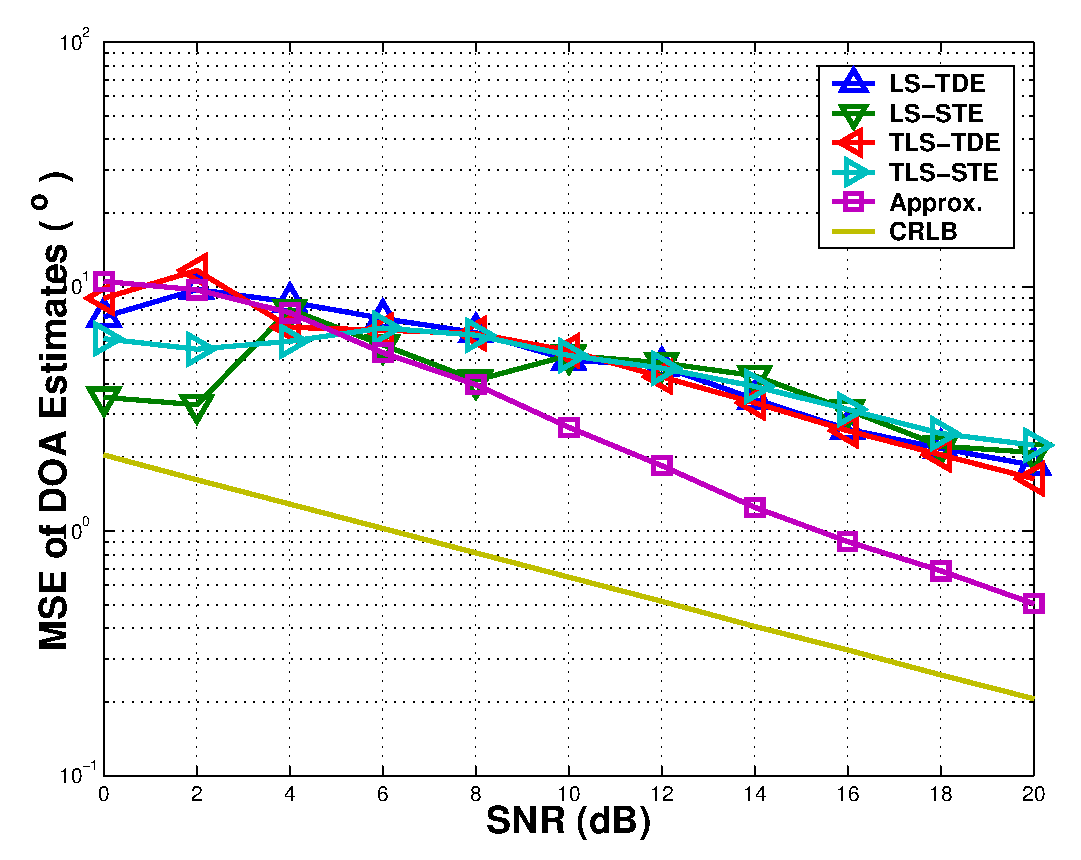
\includegraphics[width=3in]{SF_DOASNR.eps}
\caption{MSE of DOA estimates versus SNR using one doublet,
$N$=500, $L$=5, $K$=4.} \label{SF_DOASNR}
\end{center}
\end{figure}
\begin{figure}
\begin{center}
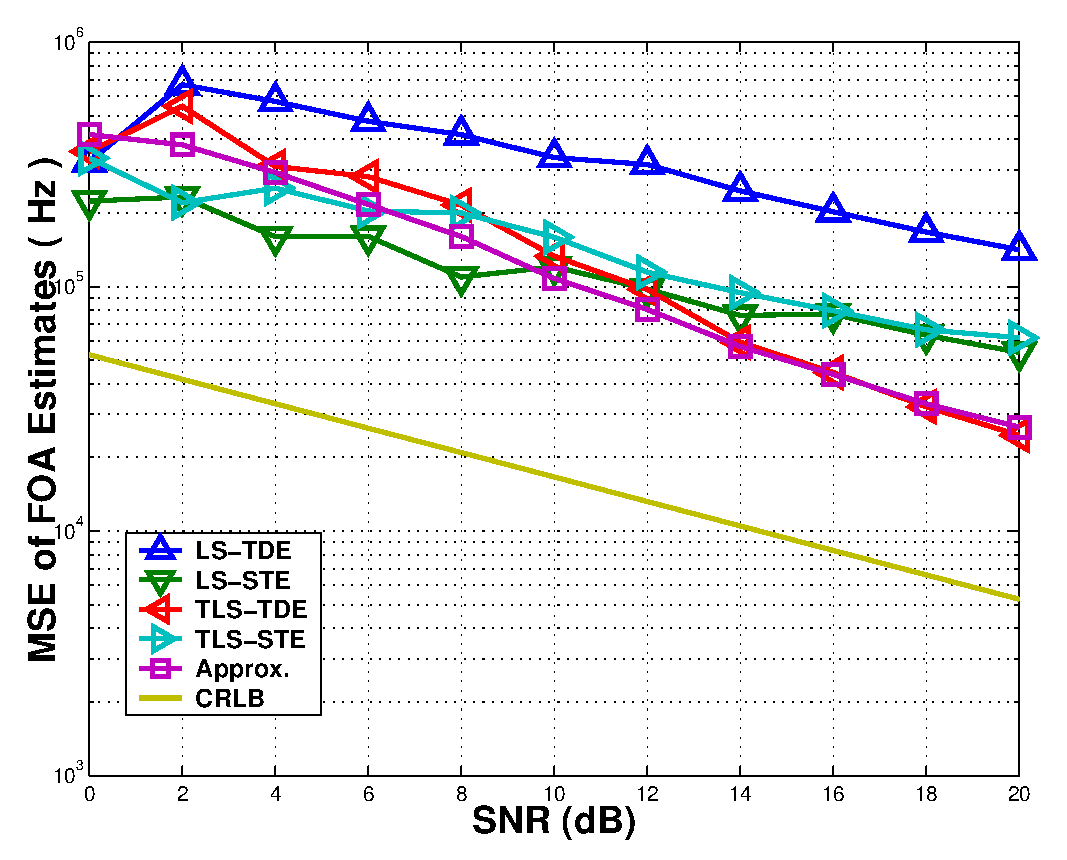
\includegraphics[width=3in]{SF_FOASNR.eps}
\caption{MSE of FOA estimates versus SNR using one doublet,
$N$=500, $L$=5, $K$=4.} \label{SF_FOASNR}
\end{center}
\end{figure}

We assume there are $M=2$ antenna elements in the array receiver,
while there are $K=4$ incoming signals. $L=5$ and $N=500$. The MSE
of the DOA/FOA estimation of the signal source ($+30^{\circ}$,
$5.5MHz$) are calculated and shown in Figs. \ref{SF_DOASNR} and
\ref{SF_FOASNR}, respectively. The MSE of the estimates are
steadily decreasing with the increase of SNR. The performance of
improved algorithms are better than LS-TDE in FOA estimation.
\subsection*{Case 2: Performance versus L}
\begin{figure}
\begin{center}
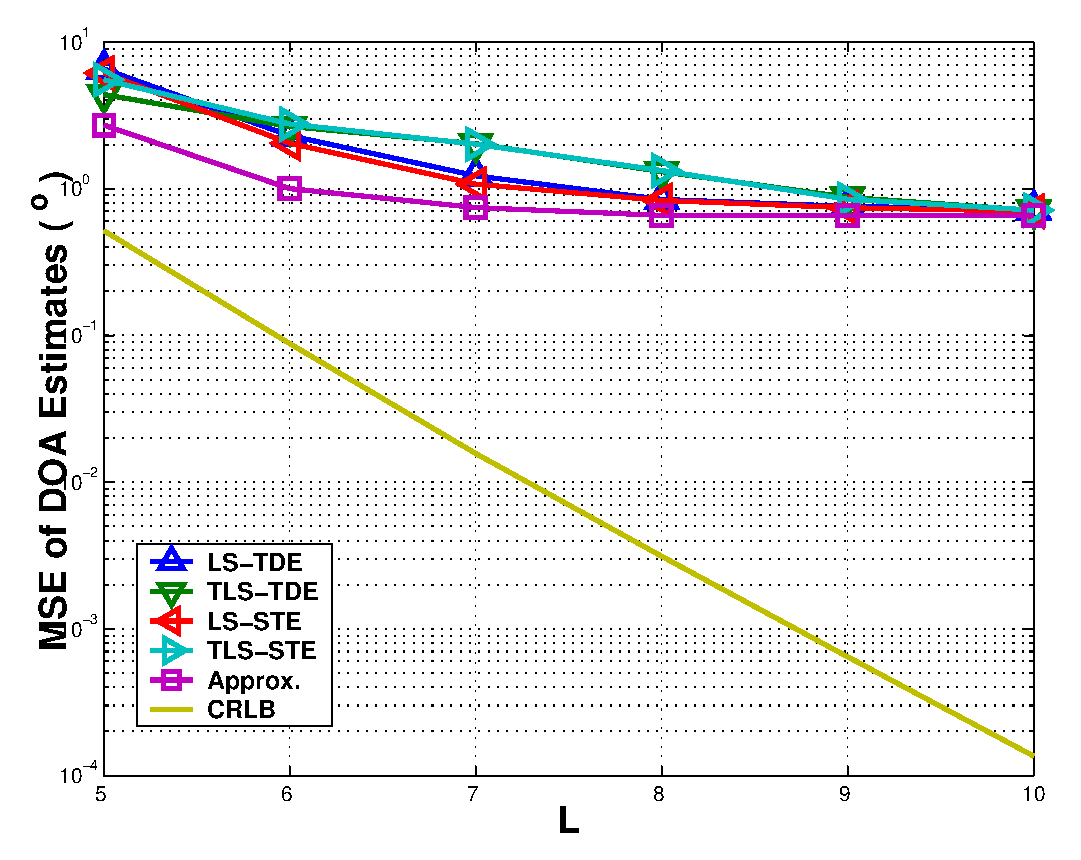
\includegraphics[width=3in]{SF_DOAL.eps}
\caption{MSE of DOA estimates versus $L$, $N$=500, $M$=2, $K$=4,
$SNR$=10dB.} \label{SFDOAL}
\end{center}
\end{figure}
\begin{figure}
\begin{center}
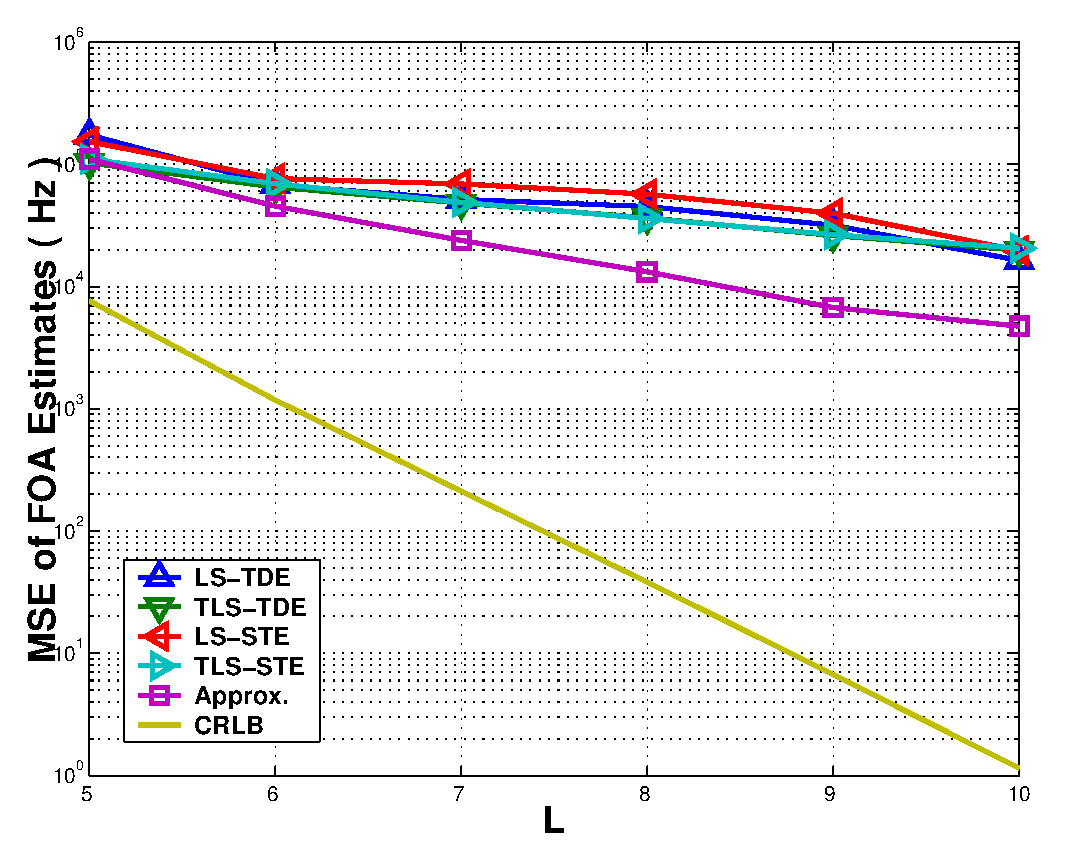
\includegraphics[width=3in]{SF_FOAL.eps}
\caption{MSE of FOA estimates versus $L$, $N$=500, $M$=2, $K$=4,
$SNR$=10dB.} \label{SFFOAL}
\end{center}
\end{figure}

In Figs. \ref{SFDOAL} and \ref{SFFOAL}, we examine the performance
of all the proposed ESPRIT algorithms with the increase of $L$.
The performance of DOA/FOA estimation becomes better. One reason
is that, with the increase of $L$, the estimation of FOA becomes
better due to more accurate subspace separation.
\subsection*{Case 3: Performance versus M}
\begin{figure}
\begin{center}
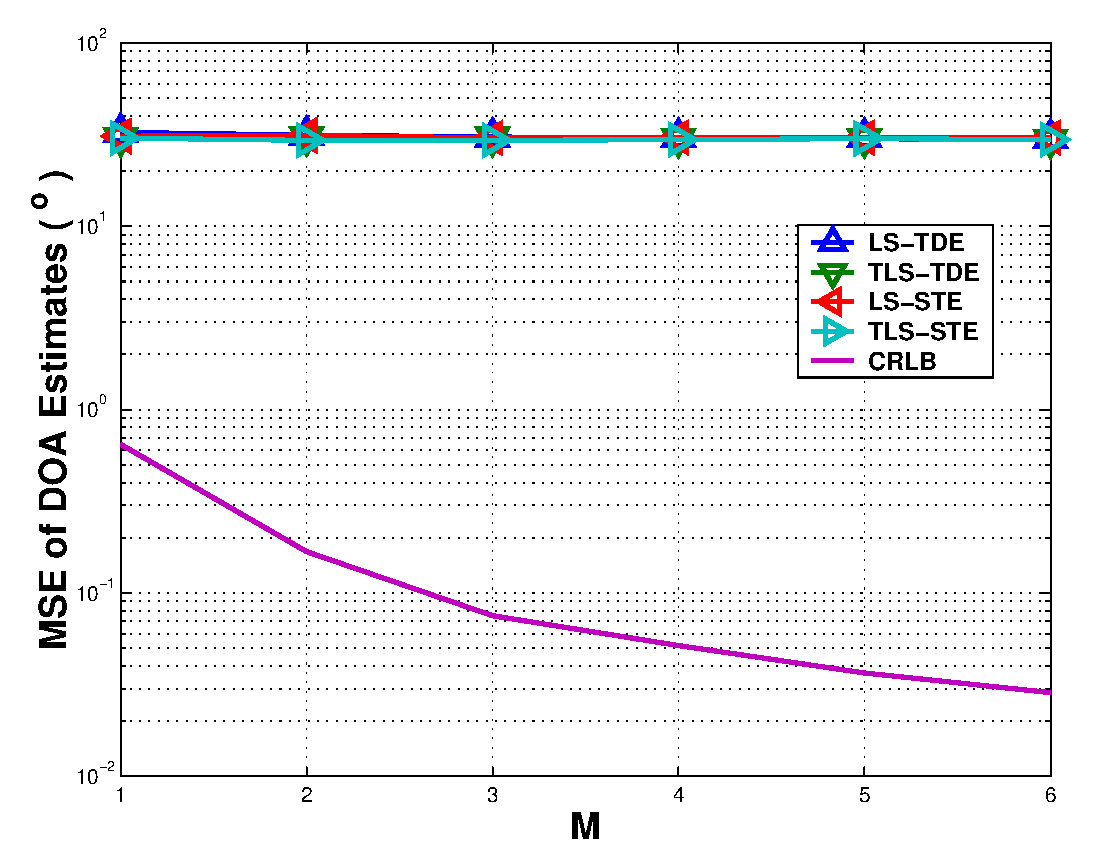
\includegraphics[width=3in]{SF_DOAM.eps}
\caption{MSE of DOA estimates versus $M$, $N$=500, $L$=5, $K$=4,
$SNR$=10dB.} \label{SFDOAM}
\end{center}
\end{figure}
\begin{figure}
\begin{center}
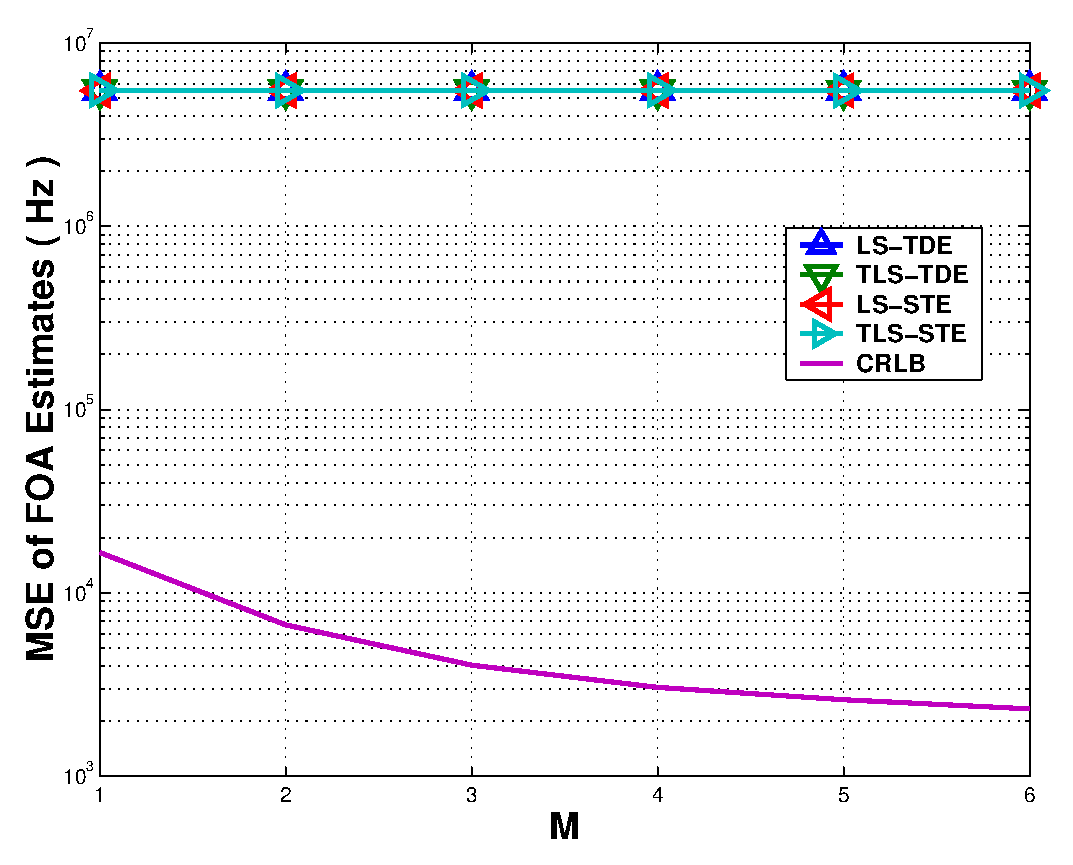
\includegraphics[width=3in]{SF_FOAM.eps}
\caption{MSE of FOA estimates versus $M$, $N$=500, $L$=5, $K$=4,
$SNR$=10dB.} \label{SFFOAM}
\end{center}
\end{figure}

In Figs. \ref{SFDOAM} and \ref{SFFOAM}, we examine the performance
of all the proposed ESPRIT algorithms with the increase of $M$.
There is no obvious change of the performance with the increase of
$M$. One reason is that the increase of $M$ is equivelant to
increase the sampling number $K$ in Eq. \ref{CorrelationXX}.
Usually, increasing $M$ cannot significantly improve the
estimation of DOA/FOA.
\section{Conclusions}

In this paper, we consider a ESPRIT array and extend the classic
ESPRIT algorithm for DOA/FOA estimation. All the proposed
algorithms are simple and direct. There are additional pairing
procedure and the number of the sources being simultaneously
estimated can be arbitrarily larger than the number of the antenna
elements to be used. In practice, this is expected to be helpful
to reduce the hardware investment.

\tiny
\bibliographystyle{unsrt}
\bibliography{GlobeCom03Array}
\end{document}
